% Chapter 1

\chapter{Introduction} % Chapter title
\label{ch:introduction} % For referencing the chapter elsewhere, use \autoref{ch:introduction} 

%----------------------------------------------------------------------------------------
\section{Summary on Optical Coherence Tomography}
\label{sec:intro}

The technique of \acf{OCT}, firstly introduced in the late 80's by \citeauthor{Fujimoto1986} \cite{Fujimoto1986} and later improved by \citeauthor{Huang1991} \cite{Huang1991}, was delevoped for the noninvasive axial and cross-sectional imaging of biological tissues.
In a way similar to ultrasonic imaging, 2D images are generated by combining the incident electromagnetic radiation with its delayed version reflected by the sample under test.\\
% OCT imaging is based on low-coherence interferometry, which employs broad bandwidth optical sources to 



The advantage over conventional ultrasound techniques is that it permits imaging resolutions
that range from 1 to 20 $\mu$m, which is up to two orders of magnitude smaller than for ultrasound. This enables the diagnonis of pathologies which were previously only detectable by histological techniques, which have the advantage of higher resolution at the expense of the capability of non-destructive measurement. In fact, histology requires the following steps to be performed on the sample:
\begin{itemize}
    \item Excision
    \item Fixation
    \item Embedding
    \item Microtoming
    \item Staining
\end{itemize}

These operations prevent the use of histology in certain areas where the sample to be analyzed cannot be damaged, such as \emph{Ophtalmology}, a field of medicine which studies the pathologies of the human eyeball and orbit. These characteristics, coupled with its real-time imaging capability, make \ac{OCT} one of the strongest candidates for this particular branch of medicine. 

In \autoref{fig:huang-oct-vs-histology} we can compare the images of a human retina obtained with the first type of OCT technique invented, \acf{TD-OCT}
(\autoref{fig:huang-oct-sub}) and histology (\autoref{fig:huang-hist-sub}) \citep{Huang1991}. Image quality, while arguably low, is enough to identify and measure the thickness of the main structures of the eye. In \autoref{fig:dhallaeyessoctsub} we can instead see a high quality image of a live sample obtained with the more modern \acf{SS-OCT} technique \citep{Dhalla2012}, which allows higher quality measurements and fast image acquisitions. \\ 

\begin{figure}[hbt]
\myfloatalign
\subfloat[OCT]
{\label{fig:huang-oct-sub}
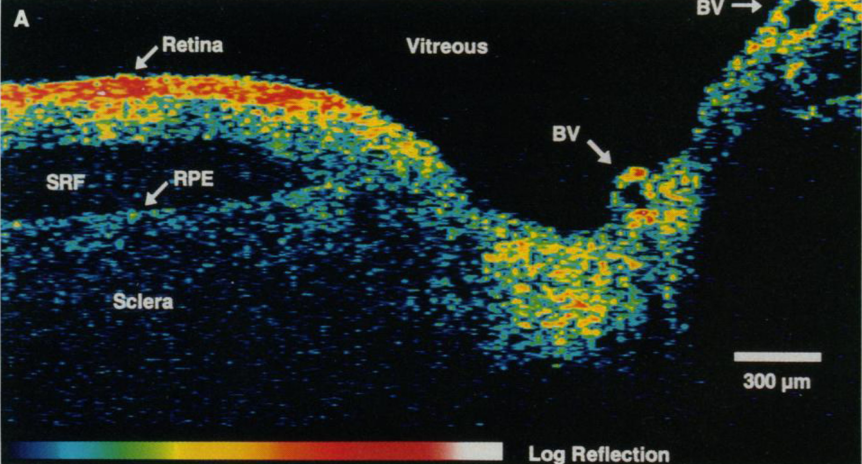
\includegraphics[width=.45\linewidth]{gfx/ch1/huang-eye}} \quad
\subfloat[Histology]
{\label{fig:huang-hist-sub}
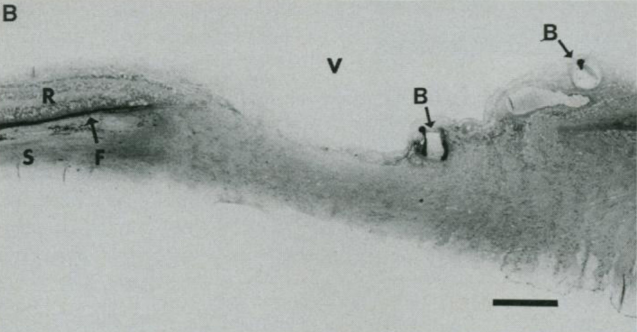
\includegraphics[width=.45\linewidth]{gfx/ch1/huang-histology}}\\
\subfloat[SSOCT]
{\label{fig:dhallaeyessoctsub}
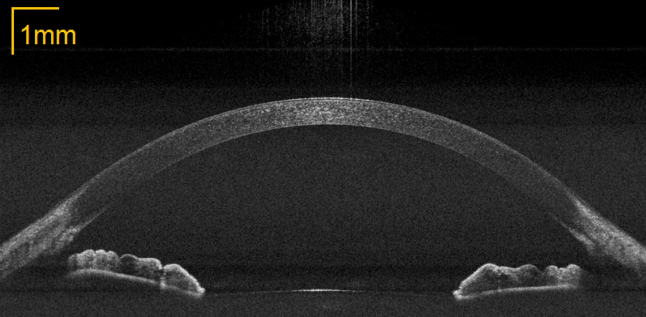
\includegraphics[width=.65\linewidth]{gfx/ch1/dhalla-eye-ssoct-2}}\\
\caption[OCT and histological images of the human eye.]{Optical coherence tomograph of human retina and optic disk in vitro (top left) and histologic section of the same sample (top right) \citep{Huang1991}. On the bottom, a \ac{SS-OCT} image of a live human eye sample \citep{Dhalla2012}. }\label{fig:huang-oct-vs-histology}
\end{figure}


The first drawback of OCT as a medical imaging technique comes from its relatively low imaging penetration, which is usually between less than a millimeter up to a couple of centimeter, depending on the specific technology and the absorption coefficient of the sample to analyse. In \autoref{fig:imaging-techniques-comparison}, a comparison between OCT, Ultrasound, and Confocal Microscopy is available \citep{Drexler2015}. The trend is that for an increasingly better imaging resolution, imaging depth has to be sacrificed. In this aspect, OCT sits right between the other two techniques, offering micrometer-level resolution for a moderate image penetration. \\

\begin{figure}[htb]
\myfloatalign
{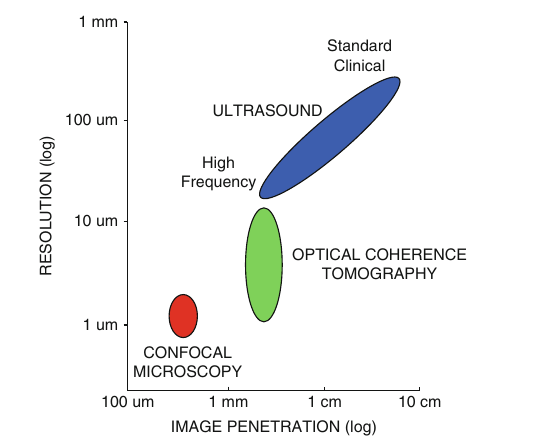
\includegraphics[width=.7\linewidth]{gfx/ch1/techniques-comparison}}
\caption{Imaging resolution and image penetration compared for different imaging techniques.}\label{fig:imaging-techniques-comparison}
\end{figure}

\begin{table}
\myfloatalign
\begin{tabularx}{\textwidth}{Xllll} \toprule
    \tableheadline{Source} & \tableheadline{Year} & \tableheadline{Voxels} & \tableheadline{Vol. Rate} & \tableheadline{Speed} \\
                           &  &  & {\scriptsize Volumes/s} & {\scriptsize GVoxels/s} \\ \midrule
    \citeauthor{Zhang10}\cite{Zhang10}             & 2010 & 6400000    & 10    & 0.06 \\
    \citeauthor{Choi2012} \cite{Choi2012}           & 2012 & 4194304    & 41    & 0.17 \\
    \citeauthor{Wieser14} \cite{Wieser14}           & 2014 & 40960000   & 26    & 1.07 \\
    \citeauthor{Darbrazi2016} \cite{Darbrazi2016}   & 2016 & 1408800000 & 2.05  & 2.89 \\
\bottomrule
\end{tabularx}
\caption{Performance of different implementations of volumetric OCT using GPGPU (adapted from \citep{Darbrazi2016}).}
\label{tab:volume-performance}
\end{table}


Whenever cross-sectional images are not sufficient for a correct diagnosis, volumetric data can be exploited for a more in-depth analysis. Volumetric images are composed by multiple 2D images captured in succession along a certain scanning direction, creating a 3D grid of datapoints called Voxels. \marginpar{A voxel is the primary unit of three-dimensional datasets, like the pixel is for 2D data. The word voxel originated by analogy with the word "pixel", with vo representing "volume" and el representing "element"} . Two examples of 3D-OCT data obtained with SS-OCT (left) \citep{Dhalla2012} and SD-OCT (right) \citep{Choi2012} are depicted in \autoref{fig:3d-example}. 

With the near-exponential growth in computing power over the last decades, and the advent of \ac{GPU} computing by means of the \ac{GPGPU} paradigm, advanced volume rendering and signal-processing algorithms can be applied on large OCT data sets in real-time. In \autoref{tab:volume-performance} a few results from the literature are summarized, highlighting the advancement in processing power using GPU solutions (adapted from \citep{Darbrazi2016}).

Starting from 3D-OCT data it is also possible to generate \emph{en-face} projections of the sample at different depths, providing an invaluable tool for further analysis. A result of this technique is available in \autoref{fig:en-face-example}, which shows a frontal view of the macula, the central part of the retina, affected by an edema.

\begin{figure}[hbt]
\myfloatalign
\subfloat[Human eye]
{\label{fig:3d-example-a}
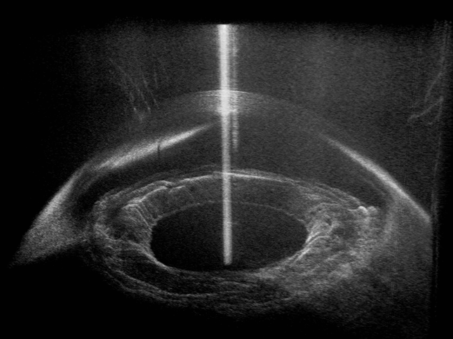
\includegraphics[height=4.5cm]{gfx/ch1/dhalla-eye-3d}} \quad
\subfloat[Human finger]
{\label{fig:3d-example-b}
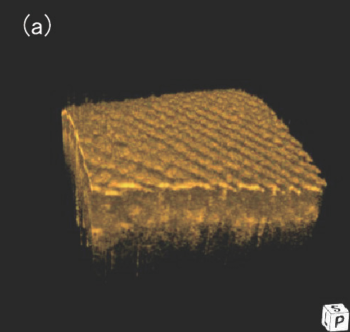
\includegraphics[height=4.5cm]{gfx/ch1/choi-finger-3d}}\\
\caption{Example of 3D OCT data: human eye obtained with SS-OCT \citep{Dhalla2012} (left) and human finger obtained with SD-OCT \citep{Choi2012} (right).}\label{fig:3d-example}
\end{figure}

\begin{figure}[hbt]
	\myfloatalign
		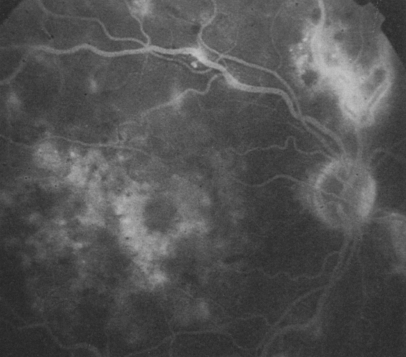
\includegraphics[width=0.45\linewidth]{gfx/ch1/en-face}
	\caption{En-face view for the assessment of macular edema \cite{MichaelRHee1995}.}\label{fig:en-face-example}
\end{figure}

% APPLICATIONS
\section{Applications}
\subsection{Medicine}
\marginpar{Angiography or arteriography is a medical imaging technique used to visualize the inside, or lumen, of blood vessels and organs of the body}
Ophtalmic applications have already been briefly mentioned in \autoref{sec:intro}, but other areas of medicine such as Cardiology \citep{Jang604,Bouma317} and Angiography \citep{Spaide2015,Jia2014} have benefitted from the diagnostic capabilities of OCT. A comparison between OCT and Ultrasound images of a coronary plaque is available in \autoref{fig:coronary}: the higher resolution of the optical system is substantial.



\begin{figure}[hbt]
	\myfloatalign
	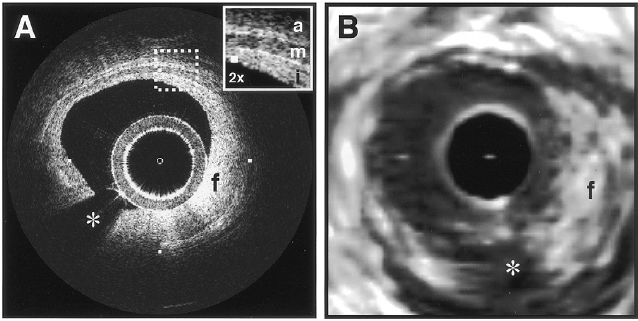
\includegraphics[height=4.5cm]{gfx/ch1/oct-vs-ultrasound-endoscopy}
	\caption{Coronary plaque imaged by OCT (left) and  \acf{IVUS} (right) \citep{Jang604}.}\label{fig:coronary}
\end{figure}


These applications are made possible by the small footprint of optical fibers (in the order of 200 $\mu$m of diameter) and the use of \ac{MEMS} mirrors, which can be easily embedded in endoscopes, catheters or other special probes \citep{Tearney96,Liao2017}. An example of a focus-adjustable probe is depicted in \autoref{fig:oct-endoscope}.

\begin{figure}[hbt]
	\myfloatalign
	\subfloat[Scheme.]
	{\label{fig:endoscope-scheme}
		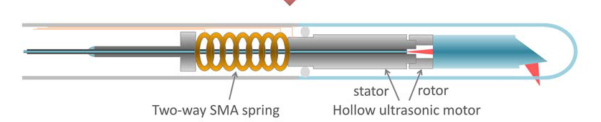
\includegraphics[width=0.55\linewidth]{gfx/ch1/endoscope-scheme}} \\
	\subfloat[Real life model.]
	{\label{fig:endoscope-real}
		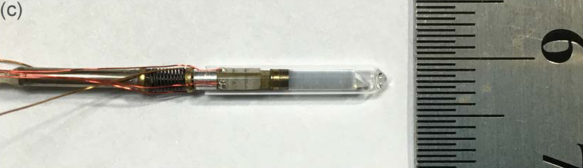
\includegraphics[width=0.55\linewidth]{gfx/ch1/endoscope-real}}\\
	\caption{Probe for endoscopic OCT \cite{Liao2017}.}\label{fig:oct-endoscope}
\end{figure}

\ac{EOCT} became an important tool for the detection of cancers affecting different parts of the human body, including bladder \citep{Xie2003}, cervix \citep{Escobar2004} and colon \citep{Hariri2006}. 
Other applications in the field of medicine include dermatology and skin damage assessment \citep{Korde2007,GAMBICHLER2005} and dentistry \citep{Amaechi2001,Machoy2017}. Low-delay, real-time OCT systems are also employed as a guidance tool for surgeries or tissue removal \cite{Boppart1999,Boppart2004}, allowing micrometer-scale resolution and providing depth-resolved images which are unobtainable with other classical methods.

\subsection{Industrial}
OCT has also found widespread application in a variety of non-medical fields, especially where non-contact, high-precision measurements are needed. For example, real-time monitoring and thickness measurement of multi-layer structures are important tools in the manufacturing of microelectronics and optical devices. Industrial uses of OCT range from defect detection in ceramic and polymeric materials \cite{Wiesauer2005,Su2014} to quality evaluation of paper products \cite{Prykari2010,Alarousu2005}. An interesting usage is found in \cite{Liang2005}, where the non-invasive examination of museum paintings was demonstrated, paving the way for OCT to the field of art conservation.

\begin{figure}[hbt]
	\myfloatalign
	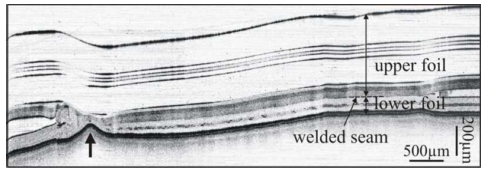
\includegraphics[width=0.5\linewidth]{gfx/ch1/material}
	\caption{Cross-sectional OCT image of a multi-layered plastic foil used in the food packaging industry \citep{Wiesauer2005}.}\label{fig:material}
\end{figure}

\subsection{In vivo monitoring of biological specimen}
We've seen that non-destructive measurements are essential in human medical diagnostic, but in vivo cross-sectional analysis is suited for a wide range of other biological samples. OCT has been used for growth monitoring of seeds \cite{Ravichandran2017}, virus detection in plants \cite{Chow2009}, and even quality assessment of egg quality in the poultry industry \cite{Sabuncu2015}. Alternative methods such as histology, \ac{SEM} imaging, \ac{MRI} and X-Ray radiography are either distructive or can not guarantee the possibility of continuous monitoring with a comparable image resolution.

\begin{figure}[hbt]
	\myfloatalign
	\subfloat[Plant seeds]
	{\label{fig:seeds}
		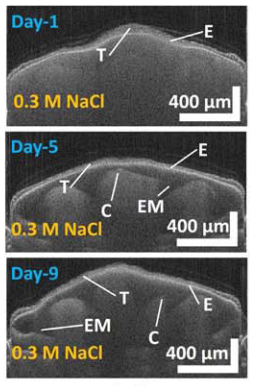
\includegraphics[height=2.5cm]{gfx/ch1/seeds}} \quad
	\subfloat[Lettuce leaf]
	{\label{fig:lettuce}
		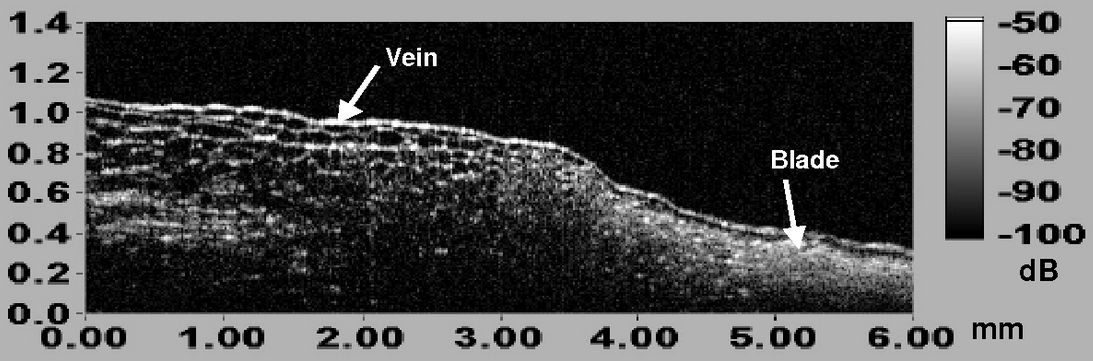
\includegraphics[height=2.5cm]{gfx/ch1/lettuce}}\\
	\caption{Growth monitoring of \emph{Capsicum annuum seeds} \cite{Ravichandran2017} (left) and lettuce leaf \cite{Loeb2003} (right).}\label{fig:plant-monitoring}
\end{figure}

\subsection{Functional imaging}
Apart from the structural imaging of biological tissue, OCT can also be utilized to perform \emph{functional} imaging, giving the user insights on the different properties of the material under analysis. \ac{PS-OCT} schemes can measure properties such as birefringence, dichroism and optic axis orientation of the sample \cite{DeBoer1997}, while \ac{DOCT} and \ac{svOCT} are able to estimate the direction and velocity of the blood flow in vessels \cite{Mahmud2013}. Birefringence measurement has found use in dentistry, specifically in the monitoring of caries lesions and their progression, enabling early detection and preventing the need for surgical intervention \cite{Fried2002}. 

\section{Objectives}
The study conducted in this thesis is based on a previous thesis \cite{Calabrese2017} developed in the \ac{PEG} Laboratory at the \ac{DEI} of the University of Padova. It consisted in the preliminary characterization of the main components of a high speed \acf{SS-OCT} system working in the 1300 nm range and the experimental determination of different parameters of the device, such as the source coherence length, the achievable scanning speed and the transversal resolution permitted by the focusing optics. \\

\noindent The primary objectives of this thesis are the following:
\begin{enumerate}
	\item Designing and testing the optical circuitry needed for a stable SS-OCT system.
	\item Developing a \ac{DAQ} application capable of continuous and low-delay video stream.
	\item Control and synchronization of the Galvanometric System with the optical source and the \ac{DAQ} board. 
	\item Acquiring cross-sectional and volumetric data of different samples.
\end{enumerate}

\section{Thesis Structure}
The structure of this document is organized in the following manner:
\begin{itemize}
	\item \autoref{ch:theory} consists of the theoretical background on the electromagnetic phenomena of interference and spatio-temporal coherence. The basic operating principle of different OCT schemes will be thoroughly detailed. 
	\item In \autoref{ch:setup} I will give a description of the optical and electrical devices that were used. I will also comprehensively describe the data flow of the \ac{DAQ} application that was developed. 
	\item \autoref{ch:results} is dedicated to explaining the methods that were used in designing the system and assessing its performance. It will also showcase a series of cross-sectional images and basic volume renderings obtained from a variety of different samples. 
	\item \autoref{ch:conclusions} concludes the thesis, illustrating possible future developments and further optimization of the presented work.  
\end{itemize}


% \begin{figure}[hbt]
% \myfloatalign
% \documentclass{standalone}


\usepackage[osf,sc]{mathpazo}
\linespread{1.05}
  \usepackage{pgfplots}
  \usepackage[euler-digits]{eulervm}
  \pgfplotsset{compat=newest}
  %% the following commands are needed for some matlab2tikz features
  \usetikzlibrary{plotmarks}
  \usetikzlibrary{arrows.meta}
  \usepgfplotslibrary{patchplots}
  \usepackage{grffile}
  \usepackage{amsmath}
  

  %% you may also want the following commands
  %\pgfplotsset{plot coordinates/math parser=false}
  %\newlength\figureheight
  %\newlength\figurewidth

\begin{document}
  \documentclass{standalone}


\usepackage[osf,sc]{mathpazo}
\linespread{1.05}
  \usepackage{pgfplots}
  \usepackage[euler-digits]{eulervm}
  \pgfplotsset{compat=newest}
  %% the following commands are needed for some matlab2tikz features
  \usetikzlibrary{plotmarks}
  \usetikzlibrary{arrows.meta}
  \usepgfplotslibrary{patchplots}
  \usepackage{grffile}
  \usepackage{amsmath}
  

  %% you may also want the following commands
  %\pgfplotsset{plot coordinates/math parser=false}
  %\newlength\figureheight
  %\newlength\figurewidth

\begin{document}
  \documentclass{standalone}


\usepackage[osf,sc]{mathpazo}
\linespread{1.05}
  \usepackage{pgfplots}
  \usepackage[euler-digits]{eulervm}
  \pgfplotsset{compat=newest}
  %% the following commands are needed for some matlab2tikz features
  \usetikzlibrary{plotmarks}
  \usetikzlibrary{arrows.meta}
  \usepgfplotslibrary{patchplots}
  \usepackage{grffile}
  \usepackage{amsmath}
  

  %% you may also want the following commands
  %\pgfplotsset{plot coordinates/math parser=false}
  %\newlength\figureheight
  %\newlength\figurewidth

\begin{document}
  \input{falloff-fit.tikz}
\end{document}

\end{document}

\end{document}

% \caption[]{Example of 3D OCT data: human eye obtained with SS-OCT \citep{Dhalla2012} (left) and human finger obtained with SD-OCT \citep{Choi2012} (right).}\label{fig:3d-example}
% \end{figure}

% \begin{figure}[hbt]
% \myfloatalign
% \documentclass{standalone}


\usepackage[osf,sc]{mathpazo}
\linespread{1.05}
  \usepackage{pgfplots}
  \usepackage[euler-digits]{eulervm}
  \pgfplotsset{compat=newest}
  %% the following commands are needed for some matlab2tikz features
  \usetikzlibrary{plotmarks}
  \usetikzlibrary{arrows.meta}
  \usepgfplotslibrary{patchplots}
  \usepackage{grffile}
  \usepackage{amsmath}
  

  %% you may also want the following commands
  %\pgfplotsset{plot coordinates/math parser=false}
  %\newlength\figureheight
  %\newlength\figurewidth

\begin{document}
  \documentclass{standalone}


\usepackage[osf,sc]{mathpazo}
\linespread{1.05}
  \usepackage{pgfplots}
  \usepackage[euler-digits]{eulervm}
  \pgfplotsset{compat=newest}
  %% the following commands are needed for some matlab2tikz features
  \usetikzlibrary{plotmarks}
  \usetikzlibrary{arrows.meta}
  \usepgfplotslibrary{patchplots}
  \usepackage{grffile}
  \usepackage{amsmath}
  

  %% you may also want the following commands
  %\pgfplotsset{plot coordinates/math parser=false}
  %\newlength\figureheight
  %\newlength\figurewidth

\begin{document}
  \documentclass{standalone}


\usepackage[osf,sc]{mathpazo}
\linespread{1.05}
  \usepackage{pgfplots}
  \usepackage[euler-digits]{eulervm}
  \pgfplotsset{compat=newest}
  %% the following commands are needed for some matlab2tikz features
  \usetikzlibrary{plotmarks}
  \usetikzlibrary{arrows.meta}
  \usepgfplotslibrary{patchplots}
  \usepackage{grffile}
  \usepackage{amsmath}
  

  %% you may also want the following commands
  %\pgfplotsset{plot coordinates/math parser=false}
  %\newlength\figureheight
  %\newlength\figurewidth

\begin{document}
  \input{falloff.tikz}
\end{document}

\end{document}

\end{document}

% \caption[]{Example of 3D OCT data: human eye obtained with SS-OCT \citep{Dhalla2012} (left) and human finger obtained with SD-OCT \citep{Choi2012} (right).}\label{fig:3d-example}
% \end{figure}

% \begin{figure}[hbt]
% \myfloatalign
% \documentclass{standalone}


\usepackage[osf,sc]{mathpazo}
\linespread{1.05}
  \usepackage{pgfplots}
  \usepackage[euler-digits]{eulervm}
  \pgfplotsset{compat=newest}
  %% the following commands are needed for some matlab2tikz features
  \usetikzlibrary{plotmarks}
  \usetikzlibrary{arrows.meta}
  \usepgfplotslibrary{patchplots}
  \usepackage{grffile}
  \usepackage{amsmath}
  

  %% you may also want the following commands
  %\pgfplotsset{plot coordinates/math parser=false}
  %\newlength\figureheight
  %\newlength\figurewidth

\begin{document}
  \documentclass{standalone}


\usepackage[osf,sc]{mathpazo}
\linespread{1.05}
  \usepackage{pgfplots}
  \usepackage[euler-digits]{eulervm}
  \pgfplotsset{compat=newest}
  %% the following commands are needed for some matlab2tikz features
  \usetikzlibrary{plotmarks}
  \usetikzlibrary{arrows.meta}
  \usepgfplotslibrary{patchplots}
  \usepackage{grffile}
  \usepackage{amsmath}
  

  %% you may also want the following commands
  %\pgfplotsset{plot coordinates/math parser=false}
  %\newlength\figureheight
  %\newlength\figurewidth

\begin{document}
  \documentclass{standalone}


\usepackage[osf,sc]{mathpazo}
\linespread{1.05}
  \usepackage{pgfplots}
  \usepackage[euler-digits]{eulervm}
  \pgfplotsset{compat=newest}
  %% the following commands are needed for some matlab2tikz features
  \usetikzlibrary{plotmarks}
  \usetikzlibrary{arrows.meta}
  \usepgfplotslibrary{patchplots}
  \usepackage{grffile}
  \usepackage{amsmath}
  

  %% you may also want the following commands
  %\pgfplotsset{plot coordinates/math parser=false}
  %\newlength\figureheight
  %\newlength\figurewidth

\begin{document}
  \input{clock.tikz}
\end{document}

\end{document}

\end{document}

% \caption[]{Example of 3D OCT data: human eye obtained with SS-OCT \citep{Dhalla2012} (left) and human finger obtained with SD-OCT \citep{Choi2012} (right).}\label{fig:3d-example}
% \end{figure}

% \begin{figure}[hbt]
% \myfloatalign
% \input{gfx/clock-1.tikz}
% \caption[]{Example of 3D OCT data: human eye obtained with SS-OCT \citep{Dhalla2012} (left) and human finger obtained with SD-OCT \citep{Choi2012} (right).}\label{fig:3d-example}
% \end{figure}

% \begin{figure}[hbt]
% \myfloatalign
% \input{gfx/clock-2.tikz}
% \caption[]{Example of 3D OCT data: human eye obtained with SS-OCT \citep{Dhalla2012} (left) and human finger obtained with SD-OCT \citep{Choi2012} (right).}\label{fig:3d-example}
% \end{figure}

% \begin{figure}[hbt]
% \myfloatalign
% \input{gfx/frequency-estimation.tikz}
% \caption[]{Example of 3D OCT data: human eye obtained with SS-OCT \citep{Dhalla2012} (left) and human finger obtained with SD-OCT \citep{Choi2012} (right).}\label{fig:3d-example}
% \end{figure}

% \begin{figure}[bth]
% \myfloatalign
% {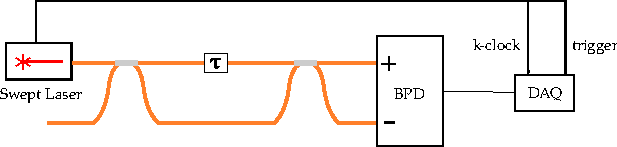
\includegraphics[width=\linewidth]{gfx/interferometer.pdf}}
% \caption{En vivo measurement of rabbit's eyeball.}
% \end{figure}


% \begin{figure}[bth]
% \myfloatalign
% {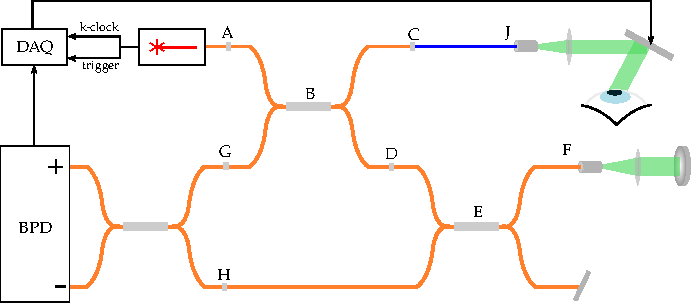
\includegraphics[width=\linewidth]{gfx/final-setup.pdf}}
% \caption{En vivo measurement of rabbit's eyeball.}
% \end{figure}

% \begin{figure}[bth]
% \myfloatalign
% {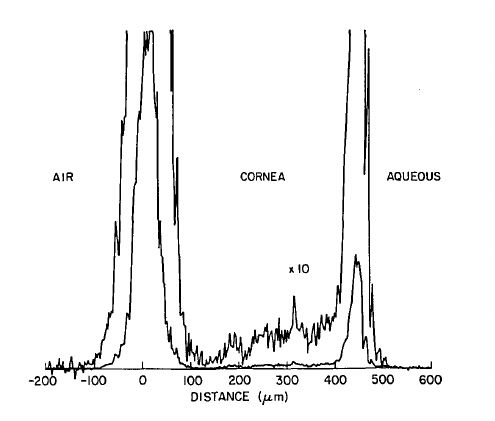
\includegraphics[width=.75\linewidth]{gfx/ch1/fujimoto-rabbit}}
% \caption{En vivo measurement of rabbit's eyeball.}
% \end{figure}

% \begin{figure}[bth]
% \myfloatalign
% \subfloat[Asia personas duo.]
% {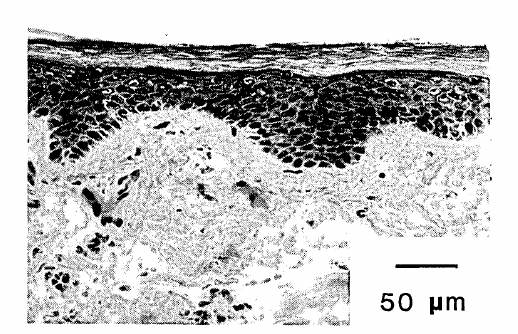
\includegraphics[width=.55\linewidth]{gfx/ch1/fujimoto-histology}} \quad
% \subfloat[Pan ma signo.]
% {\label{fig:example-b}
% 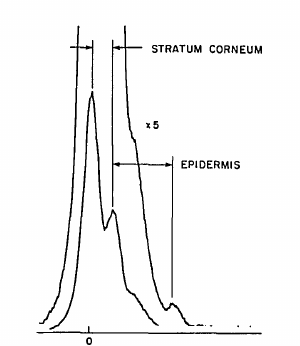
\includegraphics[width=.35\linewidth]{gfx/ch1/fujimoto-ascan}}
% \caption[Tu duo titulo debitas latente]{Tu duo titulo debitas latente.}\label{fig:example}
% \end{figure}
